\documentclass[a4paper, 12pt]{report}

\usepackage{lmodern}
\usepackage[french]{babel} % Pour la langue fran¸caise
\usepackage[utf8]{inputenc} % Pour l'UTF-8
\usepackage[T1]{fontenc} % Pour les césures des caractères accentués
\usepackage{amsmath}
\usepackage{amssymb}
\usepackage{algorithm}
\usepackage{algpseudocode}
\usepackage{graphicx}
\usepackage{calc}


\usepackage{graphicx,import,xcolor}

\newcommand{\executeiffilenewer}[3]{%
  \ifnum\pdfstrcmp%
    {\pdffilemoddate{#1}}%
    {\pdffilemoddate{#2}}%
    >0%
    {\immediate\write18{#3}}%
  \fi%
}
\newcommand{\includesvg}[2][]{%
  \executeiffilenewer{#1#2.svg}{#1#2.pdf}%
    {inkscape -z -D --file=#1#2.svg --export-pdf=#1#2.pdf --export-latex}%
  \subimport{#1}{#2.pdf_tex}%
}

\DeclareMathAlphabet{\mathcal}{OMS}{cmsy}{m}{n}
\SetMathAlphabet{\mathcal}{bold}{OMS}{cmsy}{b}{n}
\newcommand{\bigO}{\mathcal{O}}

\title{Rapport de projet ALGAV}
\author{Léo \textsc{CHECK}}


\begin{document}

\begin{titlepage}
\newcommand{\HRule}{\rule{\linewidth}{0.5mm}} 
\begin{center}
\textsc{\LARGE{}Sorbonne Université} \\[1cm]
% Logo
\includegraphics[width=0.3\columnwidth]{su.png} \\[1cm] % Logo à utiliser
\textsc{\Large{}Master Informatique} \\[0.5cm] 
\textsc{\large{}Algorithmique Avancée \\ MU4IN500} \\[0.5cm]
% Titre
\HRule \\[0.6cm]
{\huge\bfseries{}Rapport de projet} \\[0.25cm]
Rectangle et cercle minimum d'un ensemble de points \\ 
\HRule \\[1.5cm]

% Auteur
\begin{minipage}{0.45\linewidth}

\begin{flushleft}
\Large\textit{Étudiant :} \\
Léo \textsc{CHECK} % Nom auteur
\end{flushleft}
\end{minipage}
\hfill
\begin{minipage}{0.45\linewidth}
\begin{flushright}
\Large\textit{Superviseurs :} \\
M. \textsc{Danisch} \\ BM. \textsc{Bui-Xuan}  % Nom superviseur
\end{flushright}
\end{minipage} \\[2cm]

% Date
{\large 12 janvier 2020} \\[2cm] 

\end{center}
\end{titlepage}




\newpage
%===========================================================================%
\begin{small}
Les collisions entre entités est un problème courant lors de la conception d'un jeu vidéo, mais leur détection peut devenir très gourmande en ressource dès lors que la complexité et le nombre des formes géométriques augmentent. Afin de conserver des performances correctes pour l'expérience de jeu, les développeurs doivent optimiser au maximum ces opérations, notamment en utilisant des conteneurs, simplifiant grandement les calculs.
\paragraph{}
En effet, réduire les objets à des formes géométriques simples telles que les cercles et les rectangles, permet de réduire les temps de calcul étant donné que détecter leur collision se réalisent en temps constant. Cependant, ces conteneurs sont des approximations, agrandissant la réelle hitbox\footnote{masque de collision} des entités. Afin de réduire cette perte de précision, il est donc essentiel de réduire leur taille au maximum. \\
Une autre approche serait d'utiliser les enveloppes convexes. Bien plus précises, elle demande néanmoins plus de temps pour détecter la collision. En effet, étant donné un premier polygone de \emph{m} côtés et un second de \emph{n} côtés, il suffit de déterminer si un des côtés de chaque polygone se touchent. D'où une complexité en $\bigO(m \times n)$. 

L'algorithme de \emph{Toussaint} et l'algorithme de \emph{Ritter}, permettant respectivement d'obtenir un rectangle d'aire minimum et le cercle d'aire minimum d'un ensemble de points $P$, seront les cas d'études de ce rapport. Nous analyserons notamment leur efficacité et leur qualité en tant que conteneur, sur une base de test de 1664 jeux de données à 256 points, dans un plan en 2 dimensions (Varoumas). Par efficacité, nous entendons le temps de calcul nécessaire à la création du conteneur, et par qualité, l'aire du conteneur divisé par l'aire de l'enveloppe convexe : plus le rapport est petit, plus l'aire du conteneur et de l'enveloppe convexe sont proches, et donc précis.
\end{small}
%===========================================================================%
\chapter{Algorithme Toussaint}
\section{Description et analyse de l'algorithme}
L'algorithme de \emph{Toussaint} permet d'obtenir, à partir d'un ensemble $P$ de $n$ points, son rectangle d'aire minimum couvrant $R$. Il se compose en 8 étapes majeures: \\
\begin{enumerate}
\item Calculer l'enveloppe convexe de $P$, noté $HULL$.
\item Calculer les indexes des points cardinaux, notés $N$, $P$, $W$ et $E$, de l'enveloppe convexe $HULL$.
\item Construire le rectangle $R$ avec les droites $Line_N$, $Line_S$, $Line_W$ et $Line_E$ passant respectivement par $N$, $P$, $W$ et $E$.
\item Calculer l'angle minimum $\theta$ formé par une droite $Line_X$ et un côté $HULL[X] HULL[X+1]$. De plus, $X=HULL[X+1]$ (où $X \in {N,S,W,E} $).
\item Effectuer une rotation de $\theta$ des 4 droites.
\item Calculer le rectangle $R2$ avec ces dernières. 
\item Si l'aire de $R2$ est inférieure à celle de $R$, $R = R2$ (mise à jour).
\item Tant que tous les points de $HULL$ n'ont pas été traité, on effectue les étapes 4 à 6. Sinon on retourne $R$. 
\end{enumerate}

\paragraph{}
La complexité de cet algorithme dépend de plusieurs facteurs, notamment de l'implémentation du calcul de l'enveloppe convexe en étape 1. Nous choisissons ici l'algorithme de Graham. Il nécessite un tri par pixel au préalable, qui se réalise en $\bigO(n)$. Pour chaque triplet successif de points qui "tournent à droite", on retire le points du milieu. On a alors $\bigO(n+n) => \bigO(n)$. Puis, de l'étape 2 à 7, on réalise des calculs en temps constants, répétés sur les $n-1$ côtés de l'enveloppe convexe. D'où $\bigO(n)$.
Par conséquent, la complexité globale de l'algorithme de Toussaint est en $\bigO(n)$.
\\
\begin{center}
\includegraphics[width=0.5\textwidth]{ToussaintSchema.pdf}
\begin{figure}[!h]
\caption{Principe de l'algorithme de \emph{Toussaint}}
\end{figure}\end{center}

\section{Résultats}

\begin{figure}[htbp]
\centering
\begin{minipage}[t]{0.47
\textwidth}
\def\svgscale{0.45}
\input{qualityR.pdf_tex}
\caption{Qualité du conteneur rectangle d'aire minimum par instance de \emph{Varoumas}}
\end{minipage}
\hfill
\begin{minipage}[t]{0.47\textwidth}
   \
\def\svgscale{0.45}
\input{timeR.pdf_tex}
\caption{Temps de calcul (ms) par instance de \emph{Varoumas}}
\end{minipage}
\end{figure}

\paragraph{}
Nous pouvons dès à présent constater sur la figure 1.1 que la qualité du rectangle minimal sur différentes données varie peu. Avec un écart type d'environ 0.03, elle est en moyenne de 1.30. En d'autre terme, l'aire du rectangle d'aire minimal est $30\%$ plus grand que l'aire de l'enveloppe convexe en moyenne.
\paragraph{}

De plus, le temps de calcul sur les instances de données de \emph{Varoumas} est globalement constant. Le rectangle minimum d'un ensemble $P$ de 256 points est obtenu très rapidement, en 0.013 ms en moyenne.

\paragraph{}
Afin d'évaluer comment le temps de calcul croît avec la taille d'une instance de donnée, nous créons un nouvel ensemble $P_1$ de 500 000 points aléatoires. Puis, nous tirerons au hasard 256 points de $P_1$, et les stockerons dans un ensemble $P_2$. Enfin, nous mesurerons l’exécution de l'algorithme sur $P_2$ en ajoutant au hasard un autre point de $P_1$. Nous réitérerons ces opérations jusqu'à ce que $P_2$ soit de taille 100 000. \\

\begin{figure}[htbp]
\centering
\begin{minipage}[t]{0.47
\textwidth}
\def\svgscale{0.45}

\input{randomTimeR.pdf_tex}
\caption{Évolution du temps de calcul de \emph{Ritter} avec le nombre de points (nombre de l'instance = nombre de points}

\end{minipage}
\end{figure}
\paragraph{}
Le temps d’exécution de l'algorithme de \emph{Toussaint} augmente linéairement avec le nombre de points contenu dans l'instance de test, vérifiant notre analyse de complexité en $\bigO(n)$.

\chapter{Algorithme Ritter}
\section{Description et analyse de l'algorithme}
\paragraph{}
L'algorithme de \emph{Ritter} permet d'obtenir, à partir d'un ensemble $P$ de $n$ points, son cercle d'aire minimum couvrant $C$. Il se compose en 9 étapes majeures: \\
\begin{enumerate}
\item Considérer un point arbitraire $dummy$ de l'ensemble $P$.
\item Calculer un point $P$ de distance maximale à $dummy$.
\item Calculer un pojnt $Q$ de distance maximale à $P$.
\item Soit le cercle $C$ de centre $X$, de rayon $|XP|$, passant par $P$ et $Q$. 
\item Retirer de $P$ tous les points compris dans le cercle $C$
\item S'il reste des points dans $P$, $C$ n'a pas encore couvert $P$. Soit $S$ un de ces points. Sinon, on retourne $C$.
\item Tracer la droite passant par $S$ et $X$, coupant $C$ en deux points. Soit $T$, le point le plus éloigné de $S$
\item Calculer le nouveau cercle $C$ ayant pour diamètre le segment $ST$, centré en $X$ le centre de $ST$.
\item Boucler à l'étape 5.
\end{enumerate}
\paragraph{}
Dans cet algorithme, nous réalisons aux étapes 1, 4, 6, 7 et 8 des opérations en temps constant, et aux étapes 2, 3 et 5 en $\bigO(n)$ (parcours de tous les points dans $P$). Nous bouclons les étapes 5 à 8 un nombre de fois limité $a$, dépendant des points $S$ tiré à l'étape 7. En effet, en fonction de la distance $|SX|$, le nombre de points retirés à l'étape 5 à la prochaine itération sera plus ou moins grand, affectant directement la vitesse d'exécution de l'algorithme. Nous obtenons donc un algorithme $\bigO(a \times n)$. \\
Plusieurs approches nous permettraient de réduire le facteur $a$. Nous pourrions par exemple effectuer un tri par pixel de l'ensemble $P$ pour réduire sa taille, ou calculer l'enveloppe convexe de $P$ au préalable.

\begin{center}
\includegraphics[width=0.5\textwidth]{RitterSchema.pdf}
\begin{figure}[!h]
\caption{Principe de l'algorithme de \emph{Ritter}}
\end{figure}\end{center}
\section{Résultats}

\begin{figure}[htbp]
\centering
\begin{minipage}[t]{0.47\textwidth}
\def\svgscale{0.45}
\input{qualityC.pdf_tex}
\caption{Qualité du conteneur cercle d'aire minimum}
\end{minipage}
\hfill
\begin{minipage}[t]{0.47\textwidth}
   \
\def\svgscale{0.45}
\input{timeC.pdf_tex}
\caption{Temps de calcul (ms)}
\end{minipage}
\end{figure}
L'air du cercle minimum est en moyenne 19\% plus grande que celle de l'enveloppe convexe, bien meilleur que celle du rectangle minimum. Mais il est important de noter la variation importante de la qualité sur la figure 2.1. En effet, l'écart type est de 0.07, soit plus de 2 fois plus important que celui du premier algorithme.

\paragraph{}
Le temps de calcul du conteneur est constant sur les jeux de données de Varoumas. Nous obtenons ainsi le cercle minimum d'un ensemble de 256 points en 0.002 ms en moyenne.
\paragraph{}
De la même manière que pour l'algorithme de \emph{Toussaint}, nous allons évaluer comment  le temps de calcul de l'algorithme de \emph{Ritter} évolue avec le nombre de point. Notons que l'évaluation à été réalisée avec le même ensemble de point aléatoire.
\begin{figure}[htbp]
\centering
\begin{minipage}[t]{0.47
\textwidth}
\def\svgscale{0.45}
\input{randomTimeC.pdf_tex}
\caption{Évolution du temps de calcul de \emph{Toussaint} avec le nombre de points (nombre de l'instance = nombre de points}
\end{minipage}
\end{figure}
\paragraph{}
Le temps d’exécution de l'algorithme de \emph{Ritter} augmente linéairement avec le nombre de points contenu dans l'instance de test, vérifiant notre analyse de complexité en $\bigO(a \times n)$.


\chapter{Discussion}
\begin{figure}[htbp]

\centering
\begin{minipage}[t]{0.47
\textwidth}
\def\svgscale{0.45}
\input{qualityRC.pdf_tex}
\caption{Qualité des conteneurs par instance de \emph{Varoumas}}
\end{minipage}
\hfill
\begin{minipage}[t]{0.47\textwidth}
   \
\def\svgscale{0.45}
\input{timeRC.pdf_tex}
\caption{Temps de calcul (ms) des conteneurs par instance de \emph{Varoumas}}
\end{minipage}
\end{figure}
En comparant la qualité des conteneurs produits par les algorithmes de \emph{Toussaint} et de \emph{Ritter} sur les jeux de données de \emph{Varoumas}, nous pouvons relever deux points. \\
Tout d'abord, le rectangle minimum est, dans l'ensemble, le plus mauvais conteneur en terme de qualité. Nous avons, en effet, une aire couvrante 30\% plus importante en moyenne que celle de l'enveloppe convexe, contre 19\% en moyenne pour le cercle minimum. De plus, le rectangle demande 6 fois plus de temps à être calculé. \\ Pourtant, la disparité de la qualité du rectangle minimum est 2 fois plus petite que celle du cercle minimum. Dans nos expériences, la qualité des rectangles minimums est comprise entre 1.19 et 1.43, tandis que les cercles minimums entre 1.06 et 1.57.

\paragraph{}
Cependant, la qualité des conteneurs dépend directement de la "forme" du polygone à couvrir (voir figure 3.3).
\begin{center}
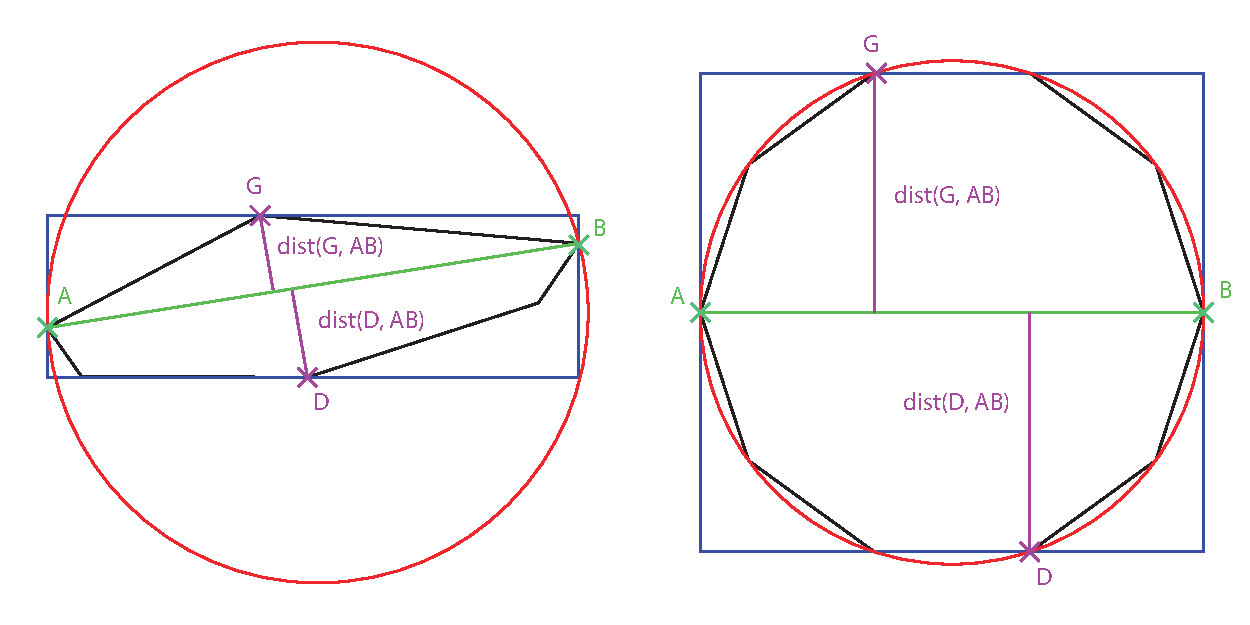
\includegraphics[width=1\textwidth]{comparaison.pdf}
\begin{figure}[!h]
\caption{Comparaison des conteneurs sur deux formes de polygones différentes}
\end{figure}\end{center}
 Il est donc important de choisir l'algorithme adéquat pour couvrir un ensemble de point $P$. \\
Une première solution serait alors de déterminer en premier temps le diamètre $AB$ du polygone (c'est-à-dire, le segment reliant les deux points les éloignés dans $P$), et $G$ (respectivement $D$) le point de $P$ le plus éloigné de $AB$ avec $\vec{AB} \wedge \vec{GB}$ maximum (respectivement $\vec{AB} \wedge \vec{AG}$ minimum). Ensuite, calculer : \[ r = |1 - \frac{|AB|}{dist(G, AB)+ dist(D, AB)}| \] \\
Ainsi, plus le rapport tend vers 1, plus la largeur et la longueur du polygone sont proches et $r$ petit. Ainsi, en fixant un $\epsilon$ jouant le rôle de délimiteur, nous pouvons soit appliquer l'algorithme de \emph{Toussaint} si $r > \epsilon$ ou de \emph{Ritter} si $r \leq \epsilon$.
\paragraph{}
Regardons à présent comment les temps de calcul des deux algorithmes évoluent avec le nombre de point sur la figure 3.4. Sur un ensemble $P$ d'environ 50 000 points ou moins, l'algorithme de \emph{Ritter} est le plus efficace. En augmentant d'avantage le nombre de point, celui de \emph{Toussaint} devient un meilleur choix en terme de performance. Évoluant tous les deux de façon linéaire comme démontré précédemment, nous pouvons clairement confirmer depuis le graphique nos analyses de complexité en  $\bigO(a \times n)$ pour le premier et en  $\bigO(n)$ pour le second. 
\begin{figure}[htbp]
\centering
\begin{minipage}[t]{0.47
\textwidth}
\def\svgscale{0.45}
\input{randomTimeRC.pdf_tex}
\caption{Comparasion de l'évolution des temps de calcul de \emph{Toussaint} et de\emph{Ritter} avec le nombre de points (nombre de l'instance = nombre de points}
\end{minipage}
\end{figure}

\chapter{Conclusion}

Les algorithmes de \emph{Toussaint} et de \emph{Ritter} permettent d'obtenir respectivement des rectangles et des cercles d'aire minimum de qualité relativement similaires d'un ensemble de point donné. De complexité $\bigO(n)$ pour le premier et $\bigO(a \times n)$ pour le second, ils évoluent de manière linéaire avec le nombre de points à traiter. Au dessus de 20 000 points,  il est préférable d'utiliser l'algorithme de \emph{Toussaint} si nous cherchons la performance. \\
Nous avons vu par ailleurs que la qualité dépend directement de la "forme" de l'enveloppe convexe de l'ensemble de point. Si nous visons la précision du conteneur, il faut savoir adapter l'algorithme utilisé. Nous avons proposé une solution qui consistait à calculer le rapport entre le diamètre de l'enveloppe convexe, et la somme des distances entre les points "les plus à gauche et à droite" au diamètre. 
\paragraph{}
Mais le problème de détection de collision ne s'arrête pas là pour les développeurs. En effet, ces algorithmes permettent seulement d'optimiser le traitement local d'une collision entre deux polygones. Dans une application réelle, nous traitons bien plus d'objets. Ainsi, dans un contexte en 2D, détecter si une collision a eu lieu entre N polygones se calcule en $\bigO(N^2)$. Différentes solutions existent : un premier exemple serait les \emph{Quad-tree}, utilisant la méthode "diviser pour régner", qui permettent de réduire la complexité à $\bigO(N \log N)$. Mais ceci reste un autre sujet d'étude.
\newpage

\bibliographystyle{}
\end{document}
